%%%%%%%%%%%%%%%%%%%%%%%%%%%%%%%%%%%%%%%%%%%%%%%%%%%%%%%%%%%%%%%%%%%
% %%%%%%%% ICML 2023 EXAMPLE LATEX SUBMISSION FILE %%%%%%%%%%%%%%%%%

% \documentclass{article}

% % Recommended, but optional, packages for figures and better typesetting:
% \usepackage{microtype}
% \usepackage{graphicx}
% \usepackage{subfigure}
% \usepackage{booktabs} % for professional tables

% % hyperref makes hyperlinks in the resulting PDF.
% % If your build breaks (sometimes temporarily if a hyperlink spans a page)
% % please comment out the following usepackage line and replace
% % \usepackage{icml2023} with \usepackage[nohyperref]{icml2023} above.
% \usepackage{hyperref}


% % Attempt to make hyperref and algorithmic work together better:
% \newcommand{\theHalgorithm}{\arabic{algorithm}}

% % Use the following line for the initial blind version submitted for review:
% % \usepackage{icml2023}

% % If accepted, instead use the following line for the camera-ready submission:
% % \usepackage[accepted]{icml2023}

% % For theorems and such
% \usepackage{amsmath}
% \usepackage{amssymb}
% \usepackage{mathtools}
% \usepackage{amsthm}
%%%%%%%%%%%%%%%%%%%%%%%%%%%%%%%%%%%%%%%%%%%%%%%%%%%%%%%%%%%%%%%%%%%%%%%%%%%%%
\documentclass[11pt]{article}
\usepackage{fullpage,url,natbib}
\usepackage{times}
\renewcommand\ttdefault{cmtt}
\usepackage{amsthm,amsfonts,amsmath,epsfig,color,float,graphicx,verbatim}
\usepackage{enumitem}
\usepackage{algorithm}
% \usepackage{algorithmic}
\usepackage{algpseudocode}
\renewcommand{\algorithmiccomment}[1]{~~~//~~#1}
\usepackage{footmisc}
\usepackage{wrapfig}
\usepackage{subcaption}
\usepackage{bbm, bm}
\usepackage{hyperref}


% Define standard colors
\definecolor{myblue}{RGB}{0,100,200}
\definecolor{lightgray}{rgb}{0.83, 0.83, 0.83}
\definecolor{white}{rgb}{1, 1, 1}
\definecolor{othergreen}{RGB}{60, 120, 0}

\hypersetup{
	colorlinks   = true, %Colours links instead of ugly boxes
	urlcolor     = blue, %Colour for external hyperlinks
	linkcolor    = myblue, %Colour of internal links
	citecolor   = othergreen %Colour of citations
}
\usepackage[table]{xcolor}


\newtheorem{theorem}{Theorem}[section]
\newtheorem*{theorem*}{Theorem}
\newtheorem{proposition}[theorem]{Proposition}
\newtheorem*{proposition*}{Proposition}
\newtheorem{example}[theorem]{Example}
\newtheorem{lemma}{Lemma}[section]
\newtheorem{corollary}[theorem]{Corollary}
% \newtheorem{assumption}{Assumption}
\newtheorem{definition}[theorem]{Definition}
\newtheorem{remark}[theorem]{Remark}
\newtheorem{assumption}[theorem]{Assumption}
\newtheorem{claim}[theorem]{Claim}
\numberwithin{equation}{section}

% we can do away with all these below commands and customize cleveref instead
% \newcommand{\secref}[1]{Section~\ref{#1}}
% \newcommand{\subsecref}[1]{Subsection~\ref{#1}}
% \newcommand{\figref}[1]{Figure~\ref{#1}}
% \renewcommand{\eqref}[1]{Eq.~(\ref{#1})}
% \newcommand{\lemref}[1]{Lemma~\ref{#1}}
% \newcommand{\thmref}[1]{Theorem~\ref{#1}}
% \newcommand{\propref}[1]{Proposition~\ref{#1}}
% \newcommand{\appref}[1]{Appendix~\ref{#1}}
% % \newcommand{\algref}[1]{Algorithm~\ref{#1}}
% \newcommand{\assref}[1]{Assumption~\ref{#1}}
% \newcommand{\defref}[1]{Definition~\ref{#1}}
% \newcommand{\corref}[1]{Corollary~\ref{#1}}


\renewcommand{\S}{\mathbb{S}}

\usepackage{bm}
\usepackage{makecell}
\usepackage{pifont}
\newcommand{\xmark}{\ding{55}}
%


\newcommand{\N}{\mathbb{N}}
\newcommand{\B}{\mathbb{B}}
\newcommand{\E}{\mathbb{E}}
\newcommand{\Z}{\mathbb{Z}}
\newcommand{\R}{\mathbb{R}}
\newcommand{\NN}{\mathbb{N}}
\newcommand{\Sbb}{\mathbb{S}}
\newcommand{\reals}{\mathbb{R}}
\newcommand{\tbg}{\tilde{\mathbf{g}}}

\newcommand{\bg}{\mathbf{g}}
\newcommand{\bx}{\mathbf{x}}
\newcommand{\bu}{\mathbf{u}}
\newcommand{\bw}{\mathbf{w}}
\newcommand{\by}{\mathbf{y}}
\newcommand{\bz}{\mathbf{z}}
\newcommand{\bDelta}{\bm{\Delta}}
\newcommand{\Unif}{\mathrm{Unif}}
\newcommand{\out}{\mathrm{out}}
\newcommand{\tf}{\tilde{f}}
\newcommand{\tvphi}{\tilde{\varphi}}
\newcommand{\tF}{\tilde{F}}
\newcommand{\norm}[1]{\left\|#1\right\|}
\newcommand{\inner}[1]{\left\langle#1\right\rangle}

%%% way too many specialized macros: 
\global\long\def\ys{y^{\star}}%
\global\long\def\ysl{y_{\lambda}^{\star}}%
\global\long\def\fxxys{\nabla_{x}f(x,\ys)}%
\global\long\def\fyxys{\nabla_{y}f(x,\ys)}%
\global\long\def\dysdx{\frac{d\ys}{dx}}%
\global\long\def\fxxysl{\nabla_{x}f(x,\ysl)}%
\global\long\def\fyxysl{\nabla_{y}f(x,\ysl)}%
\global\long\def\gxxysl{\text{\ensuremath{\nabla_{x}g(x,\ysl)}}}%
\global\long\def\gyxysl{\nabla_{y}g(x,\ysl)}%
\global\long\def\hxxysl{\nabla_{x}h(x,\ysl)}%
\global\long\def\hyxysl{\nabla_{y}h(x,\ysl)}%
\global\long\def\gxxys{\nabla_{x}g(x,\ys)}%
\global\long\def\hxxys{\nabla_{x}h(x,\ys)}%
\global\long\def\hyxys{\nabla_{y}h(x,\ys)}%
\global\long\def\gyxys{\nabla_{y}g(x,\ys)}%



\title{Fully First-Order Gradient Descent for Constrained Bilevel Optimization}

\author{}
\date{}





%%%%%%%%%%%%%%%%%%%%%%%%%%%%%%%%
% THEOREMS
%%%%%%%%%%%%%%%%%%%%%%%%%%%%%%%%
% \theoremstyle{plain}
% \newtheorem{theorem}{Theorem}[section]
% \newtheorem{proposition}[theorem]{Proposition}
% \newtheorem{lemma}[theorem]{Lemma}
% \newtheorem{corollary}[theorem]{Corollary}
% \theoremstyle{definition}
% \newtheorem{definition}[theorem]{Definition}
% \newtheorem{assumption}[theorem]{Assumption}
% \theoremstyle{remark}
% \newtheorem{remark}[theorem]{Remark}

% Todonotes is useful during development; simply uncomment the next line
%    and comment out the line below the next line to turn off comments
%\usepackage[disable,textsize=tiny]{todonotes}
\usepackage[textsize=tiny]{todonotes}

\usepackage{nicematrix}

% ========== Kai's additional package ==========
\usepackage{booktabs}
\usepackage{amsfonts}
\usepackage{amssymb,amsthm,amsmath}
\usepackage{esint}
\usepackage{isomath}
\usepackage{latexsym}
\usepackage{epic}
\usepackage{epsfig}
\usepackage{multirow}% http://ctan.org/pkg/multirow
\usepackage{hhline}
\usepackage{wrapfig}
\usepackage{verbatim}
\usepackage{enumitem}
\usepackage{color}
\usepackage{thmtools}
\usepackage{thm-restate}
% \usepackage{algpseudocode}

% \usepackage{algorithmic}
% \usepackage[ruled,vlined, linesnumbered, boxed]{algorithm2e}
\usepackage[labelformat=simple]{subcaption}
% \renewcommand\thesubfigure{(\alph{subfigure})}
% \newcommand\mycommfont[1]{\footnotesize\ttfamily{#1}}
% \SetCommentSty{mycommfont}
\usepackage{mathtools}
\usepackage{graphicx}
\usepackage{tabularx}
\usepackage{tabu}
\usepackage{colortbl}
\usepackage{breqn}
% \usepackage{minipage}

% \usepackage[labelformat=simple]{subcaption}
% \renewcommand\thesubfigure{(\alph{subfigure})}

% \newcommand{\N}{\mathbb{N}}
% \newcommand{\E}{\mathbb{E}}
% \newcommand{\Z}{\mathbb{Z}}
% \newcommand{\R}{\mathbb{R}}
% \newcommand{\NN}{\mathbb{N}}
% \newcommand{\reals}{\mathbb{R}}
% \newcommand{\bg}{\mathbf{g}}
% \newcommand{\bx}{\mathbf{x}}
% \newcommand{\bw}{\mathbf{w}}
% \newcommand{\bz}{\mathbf{z}}
\usepackage{bm}


% \newtheorem{example}{Example}
% \newtheorem{theorem}{Theorem}
% \newtheorem{definition}{Definition}
% \newtheorem{corollary}{Corollary}
% \newtheorem{proposition}{Proposition}
% \newtheorem{assumption}{Assumption}

% \newcommand{\norm}[1]{\left\lVert#1\right\rVert}

\newcommand{\gradx}{\nabla_x}
\newcommand{\grady}{\nabla_y}
\newcommand{\gradxy}{\nabla_{xy}}
\newcommand{\gradyy}{\nabla_{yy}}
% \newcommand{\L}{\mathcal{L}_{\lambda,\gamma}}
\newcommand{\yslg}{y^*_{\lambda,\gamma}}
% \newcommand{\ys}{y^*}
\newcommand{\ysg}{y^*_{\gamma}}
\newcommand{\Llg}{\mathcal{L}_{\lambda,\gamma}}
\newcommand{\weakconvexity}{\checkmark\hspace{-0.5ex}\textsubscript{w}}
\newcommand{\strongconvexity}{\checkmark\hspace{-0.5ex}\textsubscript{s}}

% =========== customized notations ============
\newcommand{\decision}{y}
\newcommand{\Decision}{\mathcal{Y}}
\newcommand{\newdecision}{z}
\newcommand{\Newdecision}{\mathcal{Z}}
\newcommand{\objective}{f}
\newcommand{\mechanism}{x}
\newcommand{\Mechanism}{\mathcal{X}}

\newcommand{\dataset}{\mathcal{D}}
\newcommand{\builder}{\mathcal{B}}

% \newcommand{\todo}[1]{{\color{red} [TODO: {#1}]}}
\newcommand{\kai}[1]{{\color{red} [Kai: {#1}]}}
\newcommand{\pswt}[1]{{\color{myblue} [SP: {#1}]}}
\newcommand{\gk}[1]{{\color{red} [Guy: {#1}]}}

\newcommand\numberthis{\addtocounter{equation}{1}\tag{\theequation}} % lets us add numbers within \[ \] env. 



% if you use cleveref..
\usepackage[capitalize,noabbrev, nameinlink]{cleveref}
\crefname{prob}{Problem}{Problems}
\crefname{eq}{Equation}{Equations}
\crefname{rem}{Remark}{Remarks}


%%%%%%%%%%%%%%%%%%%%%%%%%%%%%%%%%%%%%%%%%%%%%%%%%%%%%%%%%%%%%%%%%%%%%%
% The \icmltitle you define below is probably too long as a header.
% Therefore, a short form for the running title is supplied here:
% \icmltitlerunning{Gradient of Bilevel Optimization and Lagrangian}
%%%%%%%%%%%%%%%%%%%%%%%%%%%%%%%%%%%%%%%%%%%%%%%%%%%%%%%%%%%%%%%%%%%%%%%%
\begin{document}
%%%%%%%%%%%%%%%%%%%%%%%%%%%%%%%%%%%%%%%%%%%%%%%%%%%%%%%%%%%%%%%%%%%%%%%%%
% \twocolumn[
% \icmltitle{Gradient of Bilevel Optimization and Lagrangian}

% % It is OKAY to include author information, even for blind
% % submissions: the style file will automatically remove it for you
% % unless you've provided the [accepted] option to the icml2023
% % package.

% % List of affiliations: The first argument should be a (short)
% % identifier you will use later to specify author affiliations
% % Academic affiliations should list Department, University, City, Region, Country
% % Industry affiliations should list Company, City, Region, Country

% % You can specify symbols, otherwise they are numbered in order.
% % Ideally, you should not use this facility. Affiliations will be numbered
% % in order of appearance and this is the preferred way.
% \icmlsetsymbol{equal}{*}

% \begin{icmlauthorlist}
% \icmlauthor{Firstname1 Lastname1}{equal,yyy}
% \icmlauthor{Firstname2 Lastname2}{equal,yyy,comp}
% \icmlauthor{Firstname3 Lastname3}{comp}
% \icmlauthor{Firstname4 Lastname4}{sch}
% \icmlauthor{Firstname5 Lastname5}{yyy}
% \icmlauthor{Firstname6 Lastname6}{sch,yyy,comp}
% \icmlauthor{Firstname7 Lastname7}{comp}
% %\icmlauthor{}{sch}
% \icmlauthor{Firstname8 Lastname8}{sch}
% \icmlauthor{Firstname8 Lastname8}{yyy,comp}
% %\icmlauthor{}{sch}
% %\icmlauthor{}{sch}
% \end{icmlauthorlist}

% \icmlaffiliation{yyy}{Department of XXX, University of YYY, Location, Country}
% \icmlaffiliation{comp}{Company Name, Location, Country}
% \icmlaffiliation{sch}{School of ZZZ, Institute of WWW, Location, Country}

% \icmlcorrespondingauthor{Firstname1 Lastname1}{first1.last1@xxx.edu}
% \icmlcorrespondingauthor{Firstname2 Lastname2}{first2.last2@www.uk}

% % You may provide any keywords that you
% % find helpful for describing your paper; these are used to populate
% % the "keywords" metadata in the PDF but will not be shown in the document
% \icmlkeywords{Machine Learning, ICML}

% \vskip 0.3in
% ]
% \onecolumn
% % this must go after the closing bracket ] following \twocolumn[ ...

% % This command actually creates the footnote in the first column
% % listing the affiliations and the copyright notice.
% % The command takes one argument, which is text to display at the start of the footnote.
% % The \icmlEqualContribution command is standard text for equal contribution.
% % Remove it (just {}) if you do not need this facility.

% %\printAffiliationsAndNotice{}  % leave blank if no need to mention equal contribution
% \printAffiliationsAndNotice{\icmlEqualContribution} % otherwise use the standard text.
%%%%%%%%%%%%%%%%%%%%%%%%%%%%%%%%%%%%%%%%%%%%%%%%%%%%%%%%%%%%%%%%%%%%%%%%%%%%%%%
\maketitle

\begin{abstract}
% In this paper, we consider constrained bilevel optimization problems, where the lower level constrains are characterized by a convex function of the lower and upper variables.

% V1:
% Solving bilevel optimization is known to be challenging and often requires computing expensive Hessian due to the bilevel structure.
% Recently, a fully first-order gradient method was proposed to solve bilevel problems with stationarity guarantee, yet its result is limited to unconstrained bilevel problems only. % Background
% In this paper, we consider constrained bilevel optimization and present Fully First-order Constrained Approximation methods (F\textsuperscript{2}CA) with hyperobjective stationarity guarantee. % contribution intro
% For linear equality constraints, our algorithm can converge to an $\epsilon$-stationary solution within $O(1/\epsilon^2)$ gradient oracles, which matches to the best-known rate of the unconstrained case. % Equality summary
% For general convex inequality constraints, our algorithm constructs an inexact gradient oracle, and uses it to reach
% % an
% $(\delta,\epsilon)$-Goldstein stationarity within $\tilde{O}(\frac{1}{\delta \epsilon^4})$ first-order oracles, or $\tilde{O}(\frac{d}{\delta \epsilon^3})$ zero-order estimates where $d$ is the dimensionality of variable $x$.  % First-order and zero-order constrained
% Our experiment suggests that F\textsuperscript{2}CA demonstrates a significantly cheaper computation with a similar convergence performance compared to the Hessian-based method using differentiable optimization (\textit{cvxpylayer}).


% Our result is the first fully first-order algorithm with hyperobjective stationarity guarantees for constrained bilevel optimization problems.  % Conclusion


% Bilevel optimization is a popular yet difficult problem to solve due to the bilevel structure. Traditional methods use 

% V2:
% Solving bilevel optimization problems is known to be challenging, as most existing methods require Hessian computations which are prohibitive in modern large-scale applications.
% Recently, a fully first-order method was proposed to solve bilevel problems with finite-time stationarity guarantees, yet this result is limited only to unconstrained bilevel problems. % Background
% In this paper, we consider constrained bilevel optimization and present Fully First-order Constrained Approximation methods (F\textsuperscript{2}CA) with finite-time hyperobjective stationarity guarantees. % contribution intro
% For linear equality constraints, our algorithm converges to an $\epsilon$-stationary point within $O(1/\epsilon^2)$ iterations, matching the best-known rate in the unconstrained case. % Equality summary
% For general convex inequality constraints, our algorithm constructs an inexact hypergradient oracle, and uses it to reach
% % % an
% $(\delta,\epsilon)$-Goldstein stationarity within either $\tilde{O}(\frac{1}{\delta \epsilon^4})$ or $\tilde{O}(\frac{d}{\delta \epsilon^3})$ iterations, where $d$ is the upper-level dimension. Along the way we develop nonsmooth nonconvex optimization methods with inexact oracles, which may be of independent interest.
% We support our theoretical findings with a numerical experiment, suggesting that F\textsuperscript{2}CA demonstrates 
% similar convergence rate compared to Hessian-based methods using differentiable optimization (\textit{cvxpylayer}), while achieving significantly cheaper computation time.

Algorithms for bilevel optimization often encounter Hessian computations, which are prohibitive in high dimensions. While recent works offer first-order methods for {unconstrained} bilevel problems, \textit{constrained} bilevel optimization remains relatively underexplored. We present {the first} fully first-order constrained optimization methods with finite-time hypergradient stationarity guarantees. For linear equality constraints, our algorithm converges to an $\epsilon$-stationary point in $\widetilde{O}(\epsilon^{-2})$ gradient oracle calls, which is nearly-optimal. For general convex inequality constraints, we attain $(\delta,\epsilon)$-Goldstein stationarity in either $\widetilde{O}({\delta^{-1} \epsilon^{-4}})$ or $\widetilde{O}(d{\delta^{-1} \epsilon^{-3}})$ gradient oracle calls, where $d$ is the upper-level dimension. Along the way, we develop novel nonsmooth nonconvex optimization methods with inexact oracles. Our preliminary numerical experiments verify these theoretical convergence guarantees.
\end{abstract}



% \begin{itemize}
%     \item Kwon-inspired nonasymptotic FFO bilevel with linear equality 
%     \item Assume Lipschitzness of $F$ (hyperobjective) with a known Lipschitz constant (still a weaker assumption than, e.g. \cite{khanduri2023linearly}) and (possibly biased) zeroth order access to $F$; nonasymptotic Goldstein stationarity. 
% \end{itemize}

\section{Introduction}\label{sec:introduction}
Bilevel optimization~\cite{bracken1973mathematical, colson2007overview,bard2013practical,sinha2017review}, an important problem in optimization, is defined as follows:
\begin{align*}\numberthis\label[prob]{prob:general-constraints}
     \mbox{minimize}_{x\in \mathcal{X}} ~ F(x) \coloneqq f(x, \ystar(x)) \text{ subject to } ~\ystar(x)\in \arg\min\nolimits_{y\in S(x)} g(x, y).
\end{align*}
Here, the value of the upper-level problem at any point $x$ depends on the solution of the lower-level problem. This framework has recently found numerous applications in meta-learning~\cite{ snell2017prototypical, bertinetto2018meta, rajeswaran2019meta, ji2020convergence}, hyperparameter optimization~\cite{franceschi2018bilevel, shaban2019truncated, feurer2019hyperparameter}, and 
% continual learning~\cite{borsos2020coresets, pham2020contextual}, 
reinforcement learning~\cite{konda1999actor, sutton2018reinforcement, hong2020two,zhang2020bi}.
% , and signal processing~\cite{, , }.  
Its growing importance has spurred increasing efforts towards designing computationally efficient algorithms for it. 

As demonstrated by \cite{ghadimi2018approximation}, a key computational step in algorithms for bilevel optimization is estimating ${dy^*(x)}/{dx}$, the gradient of the lower-level solution. This gradient estimation problem has been extensively studied in differentiable optimization~\cite{amos2017optnet,agrawal2019differentiable} by applying the implicit function theorem to the KKT system of the given problem% , a technique which has found many applications in end-to-end learning \pswt{commenting out to keep the focus on the difficulty of computing the gradient}
~\cite{donti2017task,wilder2019melding,kotary2021end,lee2019meta,tang2022pyepo,bai2019deep}.
However, this technique typically entails computing (or estimating) second-order derivatives, which can be prohibitive in high dimensions~\cite{mehra2021penalty, ji2021bilevel,wang2021learning}.

Recently, \cite{liu2022bome} made a big leap forward towards addressing this computational bottleneck.  %\jz{I would not say that.}
% and is therefore not fully first-order. The convergence of first-order method using differentiable optimization is also under-investigated.
Restricting themselves to the class of unconstrained bilevel optimization, they proposed a fully first-order method with finite-time stationarity guarantees. While a remarkable breakthrough,  \cite{liu2022bome} does not directly extend to the important setting of \textit{constrained} bilevel optimization. This motivates the question: 
\begin{quote}
\centering
    \emph{Can we develop a fully first-order algorithm for constrained bilevel optimization?}
\end{quote}
Besides being natural from the viewpoint of complexity theory, this question is well-grounded
in applications, including Stackelberg models~\cite{simaan1973stackelberg,paruchuri2008playing,chu2014integrated} and mechanism design~\cite{wang2022coordinating,dutting2021optimal},  urban planning~\cite{miao2010modeling,kang2010bilevel} and resource allocation~\cite{xu2013bilevel,gutjahr2016bi,zhang2010bilevel,fathollahi2022bi}, and decision-making under uncertainty~\cite{elmachtoub2022smart,munoz2022bilevel,wilder2019melding}.
% \pswt{State a few constrained blo applications.} 
Our primary contribution is an affirmative answer to the highlighted question. While there have been some other recent works~\cite{khanduri2023linearly, yao2024constrained, lu2024firstorder} on this problem, 
 we believe our notion of stationarity more directly addresses the problem at hand
 % , 
% \jz{rephrase}\pswt{done!}
(cf. \cref{sec:related_work}).  We now summarize our contributions.
% \pswt{filler text just to see how much more space we have filler text just to see how much more space we have filler text just to see how much more space we have filler text just to see how much more space we have filler text just to see how much }
% , we answer this question affirmatively. 
% \pswt{motivate constrained bilevel as well as first-order, pose the question we answer (efficient FO constrained BLO), and segue into the next subsection}
% $S$ is a constraint set for the LL variable $y$ 

\subsection{Our contributions}\label{sec:introduction_main_results}
% We provide the following algorithmic results for constrained bilevel programs.
% \, supplementing our theory with numerical experiments.
% Our contributions can be summarized as follows:
\begin{description}[style=unboxed,leftmargin=0cm, itemsep=.5em, parsep=.3em, topsep=.5em]
\item [{(1)}] \textbf{Convex inequality constraints.} As our first contribution, we design fully first-order algorithms for solving \cref{prob:general-constraints} where the lower-level constraint set $S(x):=\left\{y:h(x,y)\leq0\right\}$  is described by convex inequality constraints, and the upper-level variable is unconstrained. 
By ``fully first-order'', we mean that we use only zeroth and first order oracle access to $f$, $g$, and $h$. 


Our measure of convergence of these algorithms is that of $(\delta,\epsilon)$-stationarity~\cite{goldstein1977optimization}: for a Lipschitz function, we say that a point $x$ is $(\delta,\epsilon)$-stationary if within a $\delta$-ball around $x$ there exists a convex combination of subgradients of the function with norm at most $\epsilon$ (cf. \cref{def:GoldsteinDeltaEpsStationary}). 

\looseness=-1To motivate this notion of convergence, we note that the hyperobjective $F$ (in \cref{prob:general-constraints}) as a function of $x$ could be nonsmooth and nonconvex (and is Lipschitz, as  we later prove). Minimizing such a function in general is well-known to be intractable~\cite{nemirovskij1983problem}, necessitating local notions of stationarity. Indeed, not only is it impossible to attain $\epsilon$-stationarity in finite time~ \cite{zhang2020complexity}, even getting \textit{near} an
approximate stationary point of an arbitrary Lipschitz function is impossible unless
the number of queries has an exponential dependence on the dimension~\cite{kornowski2022oracle}. Consequently, for this function class, $(\delta, \epsilon)$-stationarity has recently emerged to be a natural and algorithmically tractable notion of stationarity~\cite{zhang2020complexity}. We give the following guarantee under  regularity assumptions on $f$, $g$, $h$, and $y^*$. 
% \pswt{is there a word to describe the assumption on $dy^*/dx$ without going into the math? like "constraint qualification" or something?}
% Our algorithm ensures that we converge to a point that satisfies $(\delta,\epsilon)$-stationarity for $F$ in $O(\delta^{-1}\epsilon^{-3})$ iterations, each iteration costing $O(\epsilon^{-1})$.  
\begin{theorem}[Informal; \cref{thm:Lipschitz-min-with-inexact-grad-oracle} combined with \cref{thm:cost_of_computing_ystar_gammastar_inequality}]
    Given \cref{prob:general-constraints} with convex inequality constraints $S(x)=\left\{y:h(x,y)\leq0\right\}$ and unconstrained upper-level variable, under  regularity assumptions on $f$, $g$, $h$, and $y^*$ (\cref{assumption:linEq_smoothness,item:assumption_safe_constraints}), there exists an algorithm, which in $\widetilde{O}(\delta^{-1}\epsilon^{-4})$ oracle calls to $f$, $g$, and $h$, converges to a $(\delta, \epsilon)$-stationary point for $F$. 
\end{theorem} To the best of our knowledge, this is the first result to achieve fully first-order finite-time $(\delta,\epsilon)$-stationarity of the hypergradient for constrained bilevel optimization (cf. \cref{sec:related_work} for a discussion of \cite{yao2024constrained}, which recently solved a related problem). 
To this end, we begin by carefully reformulating \cref{prob:general-constraints} via the penalty method and constructing a fully first-order inexact gradient oracle for the hyperobjective $F$ (cf. \cref{sec:inequality-bilevel}). We then employ this inexact gradient oracle within {an algorithm (\cref{{alg: OIGRM}}) designed to minimize Lipschitz nonsmooth nonconvex functions}
(in particular, $F$). Our proposed algorithm offers the following convergence guarantee.
\begin{theorem}[Informal; \cref{{thm:Lipschitz-min-with-inexact-grad-oracle}}]
    Given Lipschitz $F:\reals^d\to\reals$ 
    % be Lipschitz  
% $F(\bx_0)-\inf F\leq \Delta$
and $\|\widetilde{\nabla} F(\cdot)-\nabla F(\cdot)\|\leq\epsilon$,
% Under the same setting as \citep[Theorem 7.2]{chen2023bilevel},
% suppose that $\mathrm{SGM}$ (as in \citep[Theorem 7.1]{chen2023bilevel}) is set so that $|\tF(\cdot)-\varphi(\cdot)|\leq \zeta$ for $\zeta=\Theta(\delta\epsilon/d)$.
 there exists an algorithm that, in 
% $x^{\out}$ such that $\E[\mathrm{dist}(0,{\partial}_\delta F(x^{\out}))]\leq\epsilon+\alpha$, with
$T=O(\delta^{-1}\epsilon^{-3})$
calls to $\widetilde{\nabla}F$,
% Then running \cref{alg: OIGRM} with
% $D=\Theta\left(\frac{\delta\epsilon^2}{L^2}\right),\eta=\Theta\left(\frac{\delta\epsilon^3}{L^4}\right),\nu=\delta$,
outputs a $(\delta,2\epsilon)$-stationary point of $F$.
% \pswt{Make level of detail of runtime consistent across all inf. theorems}
\end{theorem} While such algorithms using  \emph{exact} gradients already exist~\cite{zhang2020complexity, davis2022gradient}, extending them to the inexact gradient  setting is non-trivial; we leverage recent ideas connecting online learning to nonsmooth nonconvex optimization~\cite{cutkosky2023optimal} (cf. \cref{{sec:nonsmooth}}). With the ubiquity of nonsmooth nonconvex  optimization problems associated with
training modern neural networks, we believe our analysis for this general task can be of independent interest to the broader optimization community.  


% \pswt{motivate this with experiments} 
We also design variants  of the aforementioned algorithm, one of which converges in $\widetilde{O}(d_x \delta^{-1}\epsilon^{-3})$ gradient calls, thus trading off an $\epsilon^{-1}$ factor for a linear dependence on the upper dimension $d_x$, while another is 
% trading off
% Finally, we present a 
more implementation-friendly
% version of this algorithm,
with slightly worse worst-case guarantee (cf. \cref{sec:nonsmooth}).
% for full details).
% \pswt{Guy: would you be able to say a bit more about these?} \gk{Added a brief, what do you think?} <sg!

\item[{(2)}] \textbf{Linear equality constraints.} Next, we study the special setting of \cref{prob:general-constraints} with $S(x):=\left\{y:Ax - By-b=0\right\}$ a linear equality constraint and $\mathcal{X}$ a convex compact set. With appropriate regularity assumptions on $f$ and $g$, the hyperobjective $F$ in this case is smooth as a function of $x$. Inspired by ideas from \cite{kwon2023fully}, we use implicit differentiation of the KKT matrix of a slightly perturbed version of the lower-level problem to design a fully-first order approximation to $\nabla F$. With this inexact gradient oracle in hand,  we then run projected gradient descent, which converges in $\widetilde{O}(\epsilon^{-2})$ iterations for smooth functions. Constructing our first-order approximation entails solving a strongly convex optimization problem on affine constraints, which can be done efficiently (cf. \cref{sec:equality-bilevel}). 
% at a linear rate; therefore,  our total cost for achieving $\epsilon$-stationarity of $F$ is nearly-optimal at $\widetilde{O}(\epsilon^{-2})$. 

\begin{theorem}[Informal; cf. \cref{thm:lineq-cost}]
\label{thm:lineq-cost-inf}
    Given \cref{prob:general-constraints} with linear equality constraints $S(x)=\left\{y:Ax-By-b=0\right\}$ and $\mathcal{X}$ a convex compact set, under regularity assumptions on $f$ and $g$ (\cref{assumption:linEq_smoothness,assumption:eq}), there exists an algorithm, which in $\widetilde{O}(\epsilon^{-2})$  oracle calls to $f$ and $g$, converges to an $\epsilon$-stationary point of $F$. 
\end{theorem}

The current result in literature for the linearly constrained setting is that of \cite{khanduri2023linearly}, which 
involves expensive Hessian computations and 
imposes on the hyperobjective $F$ some \textit{strong regularity assumptions} that are, in general, impossible to verify.
In contrast,  we impose \textit{assumptions solely on the constituent functions $f$ and $g$} (and none directly on $F$), which can be easily verified by the user of our algorithms.
Thus, \Cref{thm:lineq-cost-inf} makes substantial progress on these two fronts.
See \cref{sec:equality-bilevel} for details. 
% \pswt{Make this distinction clearer since it's quite big, imo filler text  filler text  filler text  filler text  filler text  filler text  filler text  filler text  filler text  filler text  filler text  filler text }


% \pswt{A line about the previous best result for lineq}
\end{description}
\subsection{Related Work}

%latex note: we are using the nicematrix package to be able to get alternately shaded rows when we have multiple rows per row: this feature seems difficult to get with merely tabular (booktabs) see https://stackoverflow.com/questions/69174994/how-to-create-a-latex-table-with-specific-multicolumns-and-multirows
\begin{table}[h]
  \centering
  \resizebox{\linewidth}{!}{%
  \begin{NiceTabular}{*{11}{c}}
  \CodeBefore
  \rowcolors{1}{}{gray!10}[respect-blocks]
  \Body
    \toprule
    \Block{2-1}{\textbf{Paper}} & \Block{1-2}{\textbf{Upper Objective}} & & \Block{1-2}{\textbf{Upper Constraint}} & & \Block{1-2}{\textbf{Lower Objective}} & & \Block{1-2}{\textbf{Lower Constraint}} & & \Block{1-2}{\textbf{Cost}} \\
        \cmidrule(lr){2-3} \cmidrule(lr){4-5} \cmidrule(lr){6-7} \cmidrule(lr){8-9} \cmidrule(lr){10-11}
    & $C(x,y)$ & Smoothness & $C(x,y)$ & Smoothness & $C(x,y)$ & Smoothness & $C(x,y)$ & Smoothness & Iters. & Per Iter.\\
    \midrule
    \cite{liu2021value} & Cell 1,2.1 & Cell 1,2.2 & Cell 1,2.3 & Cell 1,3 & Cell 1,4 & Cell 1,5 & None \\
    \cite{ji2021bilevel} & --- & \checkmark & --- & --- & (, \strongconvexity) & \checkmark & --- & --- & $\kappa^3 \varepsilon^{-1}$ & Hess$\times$vec \\  
    \cite{kwon2023fully} & --- & \checkmark & \checkmark (set) & --- & (, \strongconvexity) & \checkmark & --- & --- & $\varepsilon^{-3}$ & FO \\
    \cite{chen2023near} & --- & (\checkmark, \checkmark) & --- & --- & (, \strongconvexity) & \checkmark & --- & --- & $\kappa^4\varepsilon^{-2}$ & FO \\
       \Block{2-1}{\cite{abolfazli2023inexact}} & none & (\checkmark, \checkmark) & \checkmark (set) & --- & (, \strongconvexity) & \checkmark & --- & --- & $\varepsilon^{-2}$ & mv \\
    & (\checkmark, \checkmark) & & & & & & & & $\varepsilon^{-1}$ \\
    \cite{tsaknakis2022implicit} & & & & & & & \checkmark(linear) & &  asymptotic\\ 
    \Block{4-1}{\cite{khanduri2023linearly}} & --- & (\checkmark, \checkmark) & \checkmark (set) & --- & (, \strongconvexity) & \checkmark & \checkmark (linear) & \xmark & asymptotic & --- \\
      & weak ($F$) & (\checkmark, \checkmark) & \checkmark (set) & --- & (, \strongconvexity) & \checkmark & \checkmark (linear) & \xmark & $\varepsilon^{-2}$  & \Block{3-1}{Hess$\times$vec} \\ 
      & convex  ($F$) & (\checkmark, \checkmark) & \checkmark (set) & --- & (, \strongconvexity) & \checkmark & \checkmark (linear) & \xmark & $\varepsilon^{-2}$ & \\ 
      & strongly  ($F$)  & (\checkmark, \checkmark) & \checkmark (set) & --- & (, \strongconvexity) & \checkmark & \checkmark (linear) & \xmark & $\varepsilon^{-1}$ &  \\ 
    \cite{ye2023difference} & diff. of convex & \checkmark & \checkmark (set) & --- & (\checkmark, \checkmark) & --- & (\checkmark, \checkmark) & --- &  asymptotic & \\
    \cite{gao2024moreau} & diff. of weak & & \checkmark (set) & --- & (\checkmark\hspace{-0.5ex}\textsubscript{w}, \checkmark) & \checkmark & (\checkmark, \checkmark) & & asymptotic \\
    \cite{yao2024constrained} & & \checkmark & \checkmark & \checkmark & (, \checkmark) & \checkmark & ?? \\
    \cite{DMLCBO} & --- & \checkmark & \checkmark (set) & & (, \strongconvexity) & \checkmark & \checkmark (set) & --- & $d_2^2 \varepsilon^{-4}$ & {\thead{PO, \\ inv Hess}} \\ 
    \bottomrule
\end{NiceTabular}
  }
  \captionsetup{font=scriptsize}
  \caption{All known (to us) results for two-variable bilevel problems. We use $\strongconvexity$ and $\weakconvexity$ to denote strong and weak convexity, respectively. We use $C(x,y)$ to denote the convexity in the tuple $(x,y)$. In \cite{khanduri2023linearly}, there are only smoothness assumptions on the component functions and (weak/strong) convexity assumptions on the overall smoothed implicit function $F$ (\pswt{I think this is stronger than imposing assumptions on the individual component functions making up $F$}) for nonasymptotic rates. In \cite{DMLCBO}, the $d_2$ is the dimension of the variable $y$. \pswt{Note: this table is still work in progress, and some cells are simply copied from others (when copying the corresponding rows); feel free to correct any of the cells}}
  \label{tab:distinct-columns}
\end{table}


% \begin{table}[h]
%   \centering
%   \resizebox{\linewidth}{!}{%
%   \begin{tabular}{ccccccccccc}
%     \toprule
%     \multirow{2}{*}{\textbf{Paper}} & \multicolumn{2}{c}{\textbf{Upper Objective}} & \multicolumn{2}{c}{\textbf{Upper Constraint}} & \multicolumn{2}{c}{\textbf{Lower Objective}} & \multicolumn{2}{c}{\textbf{Lower Constraint}} & \multicolumn{2}{c}{\textbf{Cost}} \\
%         \cmidrule(lr){2-3} \cmidrule(lr){4-5} \cmidrule(lr){6-7} \cmidrule(lr){8-9} \cmidrule(lr){10-11}
%     & $C(x,y)$ & Smoothness & $C(x,y)$ & Smoothness & $C(x,y)$ & Smoothness & $C(x,y)$ & Smoothness & Iters. & Per Iter.\\
%     \midrule
%     \makecell{\cite{liu2021value}} & \makecell{Cell 1,2.1} & \makecell{Cell 1,2.2} & \makecell{Cell 1,2.3} & \makecell{Cell 1,3} & \makecell{Cell 1,4} & \makecell{Cell 1,5} & \makecell{None} \\
%     \makecell{\cite{kwon2023fully}} & \makecell{Cell 2,2.1} & \makecell{Cell 2,2.2} & \makecell{Cell 2,2.3} & \makecell{Cell 2,3} & \makecell{Cell 2,4} & \makecell{Cell 2,5} & & & \makecell{$\varepsilon^{-3}$} \\
%     \makecell{\cite{chen2023near}} & \makecell{Cell 2,2.1} & \makecell{Cell 2,2.2} & \makecell{Cell 2,2.3} & \makecell{Cell 2,3} & \makecell{Cell 2,4} & \makecell{Cell 2,5} & & &  \makecell{$\varepsilon^{-2}$} \\
%       \multirow{4}{*}{\makecell{\cite{khanduri2023linearly}}} & \makecell{---} & \makecell{(\checkmark, \checkmark)} & \makecell{\checkmark (set)} & \makecell{---} & \makecell{(, strong)} & \makecell{\checkmark} & \makecell{\checkmark (linear)} & \makecell{\xmark} & \makecell{asymptotic} & \makecell{---} \\
%       & \makecell{weak ($F$)} & & & & & & & & \makecell{$\varepsilon^{-2}$} & \makecell{$\geq$Hessian} \\ 
%             & \makecell{convex  ($F$)}  & & & & & & & & \makecell{$\varepsilon^{-2}$} & \makecell{$\geq$Hessian}\\ 
%       & \makecell{strongly  ($F$)}  & & & & & & & & \makecell{$\varepsilon^{-1}$} & \makecell{$\geq$Hessian} \\ 
%   \multirow{2}{*}{\makecell{\cite{abolfazli2023inexact}}} & \makecell{none} & \makecell{(\checkmark, \checkmark)} & \makecell{\checkmark (set)} & \makecell{---} & \makecell{(, strong)} & \makecell{\checkmark} & \makecell{---} & \makecell{---} & \makecell{$\varepsilon^{-2}$} & \makecell{mv} \\
% & \makecell{(\checkmark, \checkmark)} & & & & & & & &  \makecell{$\varepsilon^{-1}$} \\
%     \makecell{\cite{ye2023difference}} & \makecell{} & \makecell{\checkmark} & \makecell{\checkmark} & \makecell{\checkmark, \xmark} & \makecell{\checkmark} & \makecell{\checkmark} & \makecell{None} \\
%     \makecell{\cite{gao2024moreau}} & \makecell{diff. of weak} & \makecell{} & \makecell{\checkmark (set)} & \makecell{---} & \makecell{(weak, \checkmark)} & \makecell{\checkmark} & \makecell{(\checkmark, \checkmark)} & & \makecell{asymptotic} \\
%     \makecell{\cite{yao2024constrained}} & \makecell{} & \makecell{\checkmark} & \makecell{\checkmark} & \makecell{\checkmark} & \makecell{(, \checkmark)} & \makecell{\checkmark} & \makecell{??}  \\
%     \bottomrule
%   \end{tabular}
%   }
%   \caption{All Known (to us) Results for Two-Variable Bilevel Problems. We use $C(x,y)$ to denote the convexity in the tuple $(x,y)$. In \cite{khanduri2023linearly}, there are only smoothness assumptions on the component functions and (weak/strong) convexity assumptions on the overall smoothed implicit function $F$ for nonasymptotic rates. \pswt{Note: this is still work in progress, feel free to correct any of the cells}}
%   \label{tab:distinct-columns}
% \end{table}

\paragraph{Lagrangian Approximation of the Hyperobjective}
Interestingly, so far, this has been the only approach to achieving truly Hessian-free algorithms. \pswt{This (not-yet-fully verified) assertion is based on me currently not understanding how \cite{yao2024constrained} is claimed to be  "hessian-free".} This remarkable breakthrough was achieved by \cite{kwon2023fully} who reformulated the given problem into a Lagrangian form, and with some very simply --- but  clever --- observations, were able to perform hypergradient updates by using \emph{exclusively first-order components}! Their rate was $\varepsilon^{-3}$ iterations, each performing only gradient computations. \pswt{note: the true dependence on $\kappa$ and polylog factors isn't shown here; see \cite{chen2023near} for this.} In another remarkable paper, \cite{chen2023near} did a more careful analysis of the algorithm and technique in \cite{kwon2023fully} to get the optimal number of iterations $\varepsilon^{-2}$. At the heart of \cite{kwon2023fully}'s novelty is a first-order approximation of the hypergradient. \pswt{To extend this to our setting, can we get a similar first-order approximation of the \emph{projected} hypergradient?}

\cite{landry2019differentiable}: no complexity analysis. 

% \cite{kwon2023fully} ($\epsilon^{-3} \log {\frac{1}{\epsilon}}$) and \cite{chen2023near} ($\epsilon^{-2} \log {\frac{1}{\epsilon}}$)

\paragraph{Smoothing the Lower-Level Solution.}
The gradient of the solution $y^\ast(x)$ of the lower-level problem plays a central role in the hypergradient (i.e., gradient of the overall objective). However, one cannot in general assume $y^\ast(x)$ to be differentiable. Some papers impose assumptions on the lower-level objective (and constraint, if needed) so that they can obtain this differentiability for free; others (which we discuss in this subsection) achieve this property via some kind of smoothing. So far, we have observed two kinds of smoothing: one via inf-convolution (also called Moreau envelope) and the other via random perturbation (e.g., \cite{khanduri2023linearly} and \cite{DMLCBO}.). We discuss these approaches below. 

The work of \cite{liu2021value} studies $\min_{x\in \mathcal{X}, y^\ast(x)\in \arg\min f(x,y)\leq 0} F(x, y^\ast(x))$, assuming only continuous differentiability of $F$ and $f$. Conceptually, the paper performs a very simple algorithm: reformulate the problem as one requiring $y$ be in the set $f(x, y) - \min_y f(x, y)\leq 0$, then uses inf-convolution to smoothen $\min_y f(x, y)$. It then transforms the bilevel problem into a single-level one by incorporating the (smoothed) constraint into the objective via a \emph{barrier} function, as is done in interior-point methods. Finally, it uses inf-convolution again to smoothen the resulting objective function of $x$. The algorithm therefore iteratively performs the following sequence of steps: first, compute the minimizer of the smoothed lower-level constraint; second, find the minimizer (with respect to $y$) of the smoothed barrier objective; third, we take a gradient step (with respect to $x$) on the smooth barrier objective. This whole subroutine is then run in the IPM framework. The paper does not provide a non-asymptotic convergence guarantee, but their technique of smoothing via inf-convolution is used in many other papers, and in what follows, we describe some of the most relevant such works. 

First, we note the work of \cite{ye2023difference}, which performs a ``value function smoothing'' via inf-convolution, then notes that the resulting problem is a difference of convex functions. It then uses established techniques from the DC programming literature to solve this problem. The paper provides asymptotic convergence guarantees. 

The (very) recent work of \cite{gao2024moreau} extends the work of \cite{ye2023difference} by removing the convexity assumption on the second variable of the lower-level problem. To do so, the paper proves weak convexity of the Moreau envelope. \pswt{To check: \cite{davis2019stochastic} already proved that the Moreau envelope of any weakly convex function is smooth with Lipschitz continuous gradient; doesn't this already imply weak convexity of the Moreau envelope? Specifically, doesn't Lemma $2.2$ of \cite{davis2019stochastic} subsume Theorems $2$ and $3$ of \cite{gao2024moreau}?} The paper provides asymptotic guarantees (see Theorem $18$).

Another similarly relevant paper that also falls under the framework of ``value function smoothing'' is that of 
  \cite{yao2024constrained}, which studies \[\min_{x\in \mathcal{X}, y^\ast(x)\in \arg\min_{y\in \left\{\mathcal{Y}\cap g(x, y)\leq 0\right\}} f(x,y)} F(x, y^\ast(x)),\] which is essentially identical to our setup. The paper's first idea is to incorporate the lower-level constraint $g(x,y)\leq0$ into the lower-level objective via a Lagrange multipler they call $\lambda$ \pswt{(note that they seem to consider $\lambda$ to be a variable independent of $x$: is this valid?)} and then using the same inf-convolution as in \cite{liu2021value} to smoothen $\min_{y\in \mathcal{Y}} f(x,y) + \lambda g(x,y)$. One key innovation is to bound $\lambda$ in the optimization used in the smoothening process. \pswt{(Note: What is the justification for this bound? How can we ensure that we will not miss the correct $\lambda$ by imposing this bound?)} The algorithm then proceeds iteratively, performing the following sequence of steps: first, it computes the minimizer of these two inf-convolutions with the current $x$, $y$, and $z$; second, it updates $x$ and $y$; third it updates $z$. \pswt{The operation of updating $x$ and $y$ is performed via a projection onto the set $\left\{y\in \mathcal{Y}| g(x, y)\leq 0\right\}$. Would the final runtime not have to consider the cost of this operation? Can we ensure it is Hessian-free, as the title claims the paper to be?} Also, \pswt{This is the only paper that \emph{claims} what our goal is; so we would need to definitely write down their correct runtime in order for us to be able to compare with them}

  Another approach to smoothing is seen in the work of \cite{khanduri2023linearly}. The authors perform a slightly different kind of smoothing, by using random perturbation. Overall, their algorithm is as follows: randomly perturb the lower-level objective, then compute the $y^\ast(x)$ corresponding to this perturbed lower-level (linearly constrained) problem. The perturbation enables differentiability of $y^\ast(x)$ (note that the expression for $\nabla_x y^\ast(x)$ has the optimal lower-level Lagrangian in it; in this setting, because the lower-level constraint is linear, the authors are able to get a closed-form expression for it \pswt{Note: the authors seem to provide a very in-depth analysis of the conditions required for differentiability of $y^\ast(x)$; I wasn't able to see such in-depth proofs in other papers, all of which use the differentiability of $y^\ast(x)$}), which is then used in computing the hypergradient; the variable $x$ is then updated using this hypergradient. The authors provide nonasymptotic rates by imposing additional assumptions of weak convexity/convexity/strong convexity on the hyperobjective obtained by perturbed smoothing. The authors also show "closeness" of the perturbed smoothed hyperobjective from the true hyperobjective. \pswt{My main concern is that the authors do not seem to have proved \emph{under what conditions on the original problem} can one see this imposed assumption on the perturbed smoothed objective $F$. Without such a proof, wouldn't their theorem be essentially incomplete?} 

  In \cite{DMLCBO}, the authors consider bilevel optimization with both upper and lower level constraints, the constraints given as explicitly defined convex sets. The authors use a closed-form formula for the hypergradient citing a result from \cite{blondel2022efficient}. Note: \pswt{This expression requires the computation of the inverse of a product of a matrix with a Gaussian-smoothed projection operator}. Instead of using the true projection operator, they use a Gaussian-smoothed version of it, thus incurring an extra dimension factor in the smoothness constant. The convergence metric used is like a gradient mapping of the projection.\pswt{Is their proof of Lemma 6 correct?}    
 
\paragraph{Projection-Free Approaches}
There has been some attempt at developing projection-free algorithms for various versions of bilevel optimization. Below, describe as many approaches as possible. 

In \cite{abolfazli2023inexact}, the authors consider $\min_{x\in \mathcal{X}, y^\ast(x)\in \arg\min_y g(x,y).} f(x, y^\ast(x))$. Note that the constraint here is in the \emph{upper-level} problem, unlike what we are considering. They assume the lower-level objective to be strongly convex and smooth; they assume the upper-level objective to be smooth, providing results for both convex and nonconvex assumptions on $f$. 
% \pswt{Note I found their assumptions somewhat difficult to parse (I believe they are all fine, just a bit technically dense for me)}. 
Their algorithm is very natural: They compute the hypergradient, followed by updating $x_k$ via Frank-Wolfe (to ensure feasibility in $\mathcal{X}$), followed by updating $y_k$ (which approximates $y^\ast(x_k)$) via a gradient step on $g$. While the naive approach to the first step (taking a gradient step on the hyperobjective) would require an expensive matrix inversion, the authors come up with a simple new idea (presented in their equations $7a$ and $7b$) that essentially changes the order of operations in the naive approach; this circumvents the expensive operations from the naive approach. We note two important points here: First: \pswt{Their equations $7a$ and $7b$, which are two slightly new steps show up in Proposition $1$ of \cite{ji2021bilevel} as well.} Second: \pswt{Given the overall nonconvexity, wouldn't convergence heavily rely on very accurate initialization, and wouldn't the stationary guarantee be weak-ish? I'm also very confused about the fact that Lemma $2.1$'s ``Lipschitz/smoothness constants" look really bad (i.e., square of some condition number), but somehow those bad constants disappear in the final iteration cost (e.g., see the proof of Corollary $4.2$) and are omitted in the results table.} 
\input{src/problem}
% \subsection{Differentiable optimization and non-fully first-order baseline}
% More precisely, ~\cite{amos2017optnet} propose treating KKT conditions of the constrained optimization problem as a fixed point equation of the optimal primal $y^*$ and dual $\gamma$ solution, and applying implicit function theorem to compute the derivative $\frac{\partial y^*}{\partial x}$ and $\frac{\partial \gamma}{\partial x}$. However, differentiating through the KKT conditions involves second-order derivatives. 

% \pswt{do we use this stuff below? it does not seem like it's used later, so we can perhaps remove it.} \kai{I think we should keep all the KKT conditions related derivation here. Later we just refer back to Section 2 for that. Some of these can be simplified to save space though.}
% \begin{align}
%     & \nabla_y g(x,y^*) + \gamma^\top \nabla_y h(x,y^*) = 0 \label{eqn:first-order-gradient} & \text{and} \quad \gamma h(x,y^*) = 0 
% \end{align}
% By computing the derivative of Equation~\ref{eqn:first-order-gradient} and applying implicit function theorem, we get a linear system of $\frac{d y^*}{d x}$ and $\frac{d \gamma}{d x}$ that can be written in a matrix form:
% \begin{align}\label{eqn:kkt-system}
% \underbrace{
% \begin{bmatrix}
% \nabla^2_{yy} g + \gamma^\top \nabla_{yy}^2 h & \nabla_y h_S^\top \\
% \text{diag}(\gamma) \nabla_y h_S & 0
% \end{bmatrix}}_{H_{\text{ineq}}}
% \begin{bmatrix}
%     \frac{\partial y^*}{\partial x} \\
%     \frac{\partial \gamma_S}{\partial x}
% \end{bmatrix}
% = 
% -
% \begin{bmatrix}
%     \nabla^2_{xy} g + \gamma \nabla_{xy}^2 h \\
%     \text{diag}(\gamma_S) \nabla_x h_S
% \end{bmatrix}
% \end{align}
% where $S$ denotes the set of active constraints $S = \{ i: h_i(x,y^*) = 0 \}$. We notice that the inactive constraints ($i \in \bar{S} = \{ h_i(x,y^*) < 0 \}$) must have zero dual solution $\gamma_i$ and zero dual derivative $\frac{d \gamma_i}{d x}$ (see Appendix~\ref{sec:inactive-constraints-in-differentiable-optimization} for more details), which can be removed in the matrix form.

% For equality constraints, we get a similar expression where all the constraints are active:
% \begin{align}\label{eqn:linear-kkt-system}
% \underbrace{
% \begin{bmatrix}
% \nabla^2_{yy} g + \gamma^\top \nabla_{yy}^2 h & \nabla_y h^\top \\
% \nabla_y h & 0
% \end{bmatrix}}_{H_{\text{eq}}}
% \begin{bmatrix}
%     \frac{\partial y^*}{\partial x} \\
%     \frac{\partial \gamma}{\partial x}
% \end{bmatrix}
% = 
% -
% \begin{bmatrix}
%     \nabla^2_{xy} g + \gamma \nabla_{xy}^2 h \\
%     \nabla_x h
% \end{bmatrix}
% \end{align}

% \cref{eqn:kkt-system} and \cref{eqn:linear-kkt-system} give a valid expression to compute subgradient $\frac{\partial y^*}{\partial x}$ under different constraints, which can be used in \cref{eqn:inequality_reformulation}.

\input{src/penalty-method}
\input{src/computation}
\input{src/inexact_oracle_algorithm}
%%% SUBSUMED BY OTHER SECTIONS %%%

\section{An Attempt via Nonconvex Nonsmooth Optimization}\label{sec:ncns_blackbox}
The objective $F$ in the lower-level constrained bilevel problem, \cref{prob:orig_bilevel},
is nonsmooth and nonconvex in $x$. In this section, we, therefore, propose solving \cref{prob:orig_bilevel} using recent developments in nonsmooth nonconvex optimization. A crucial requirement to be able to use these developments is that $F$ be Lipschitz. \pswt{note: the algorithm of DDLPY requires only Lipschitzness of the objective in question; is it possible that we can therefore get a result for the following setting: Lipschitz upper-level objective, ??? lower-level problem. Note that here we require no convexity or smoothness assumptions on the upper-level objective, something we've not seen thus far. Of course, the guarantee will also be only for Goldstein stationarity.}
\begin{lemma}\label{lem:LipscConstrBilevel}
$F$ is Lipschitz
\end{lemma}
\begin{proof}[Lipschitzness of Bilevel \pswt{check!}]
    By Lemma $2.1b$ of \cite{ghadimi2018approximation}, the hypergradient of $F$ computed with respect to the variable $x$ may be expressed as $\nabla_x F(x) = \nabla_x f(x, y^\ast(x)) + \nabla_x y^\ast(x) \cdot \nabla_y f(x, y^\ast(x))$. If we impose Lipschitzness assumptions on $f$, with respect to each of the coordinates, and additionally, if we can show $\|\nabla_x y^\ast(x)\|\leq L_{yx}$ for some constant, then it concludes the proof of Lipschitzness of $F$ with a Lipschitz constant $L_F \leq L_{fx} + L_{fy}\cdot L_{yx}$. Note that a bound on $\|\nabla_x y^\ast(x)\|$ was obtained by \cite{ghadimi2018approximation} in terms of second-order properties of $g$ and one in terms of constants from weaker assumptions in \cite{kwon2023fully} --- however, the latter also involves the Lagrange multiplier used therein. \pswt{How can we get for $y^\ast(x)$ a Lipschitz constant that is independent of any Lagrange multipliers? I think this is perhaps a self-contained question: what is the Lipschitz constant of the minimizer of a (strongly) convex function over the $0$-level set of a (strongly) convex function? Note: Jimmy has a solution for this.} 
\end{proof}
% \input{src/linear}
\section{Experiments}

\begin{figure}
    \centering
    \begin{subfigure}[b]{0.32\textwidth}
        \centering
        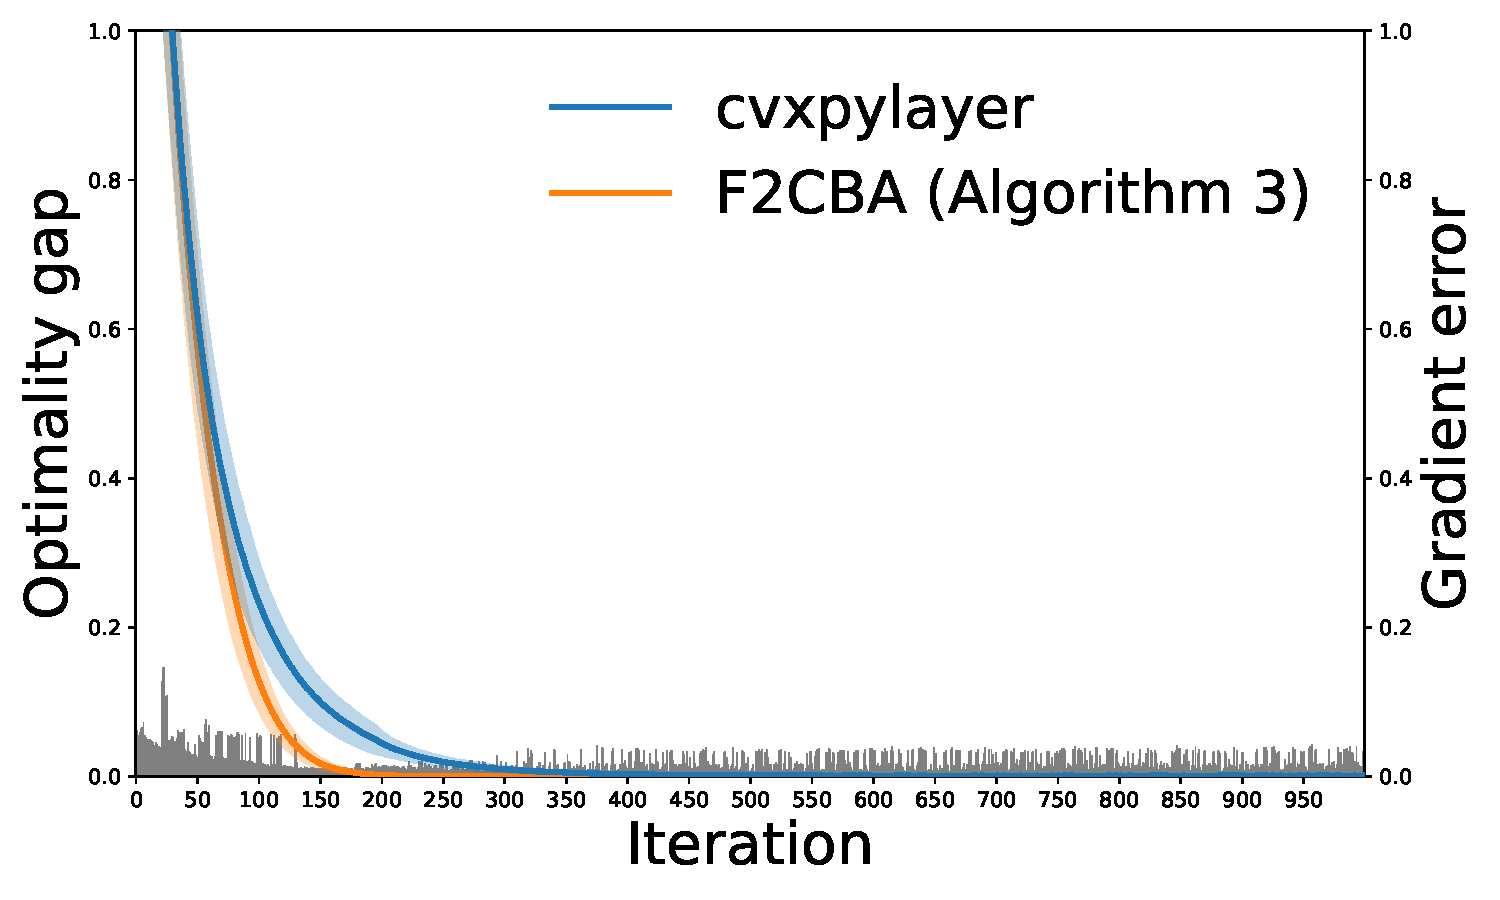
\includegraphics[width=\textwidth]{src/figures/ydim200_loss.pdf}
        \caption{Convergence comparison and gradient error plot.}
        \label{fig:convergence-comparison}
    \end{subfigure}
    \hfill
    \begin{subfigure}[b]{0.32\textwidth}
        \centering
        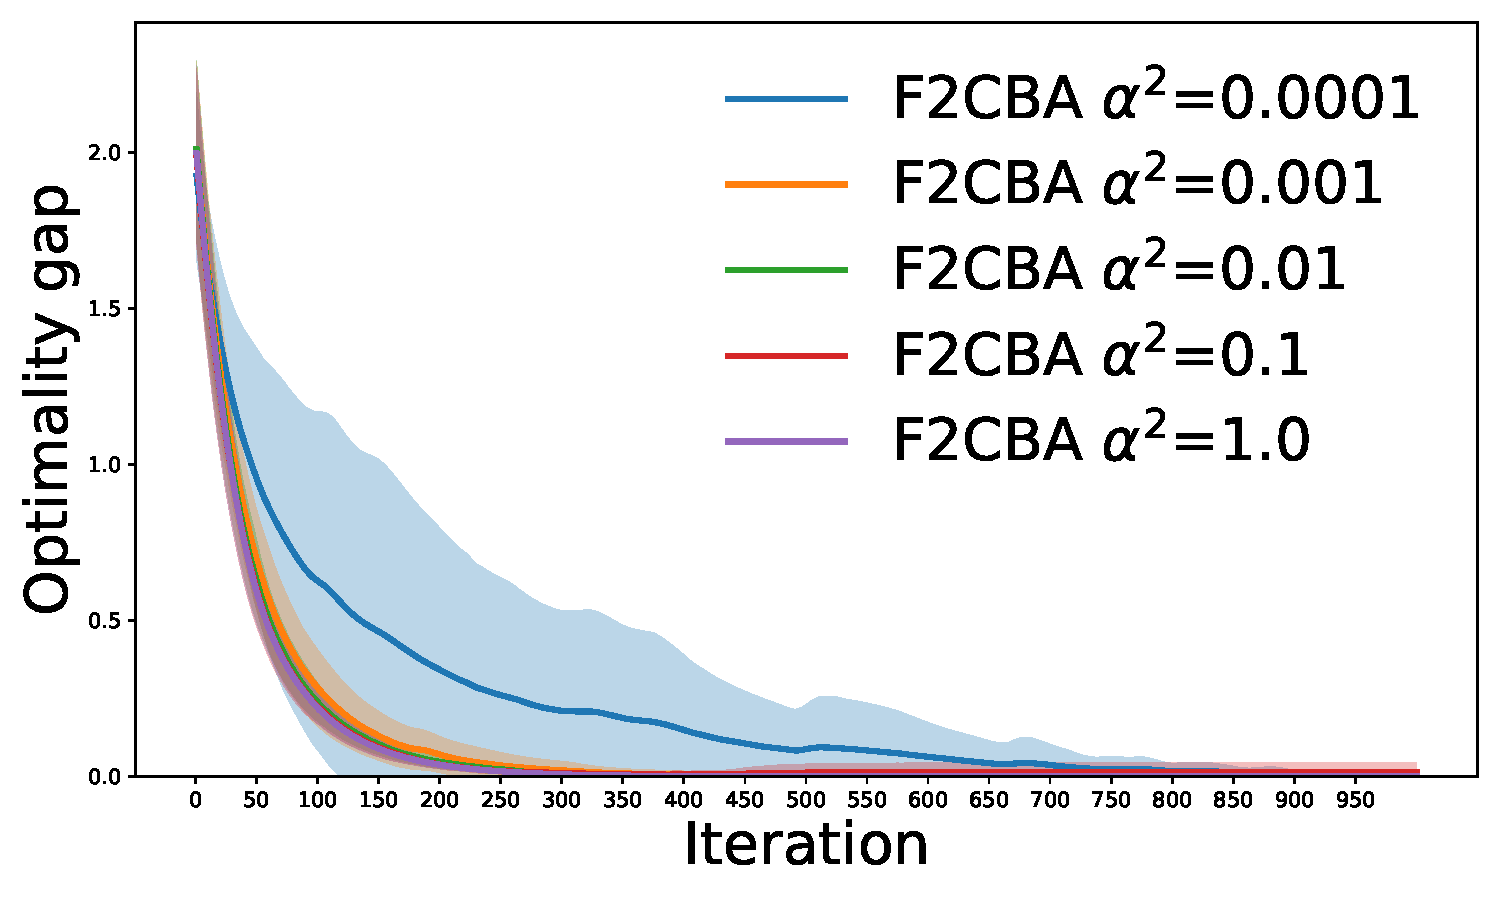
\includegraphics[width=\textwidth]{src/figures/ydim200_gradient_error.pdf}
        \caption{Convergence analysis with varying gradient inexactness $\alpha$.}
        \label{fig:convergence-comparison-2}
    \end{subfigure}
    \hfill
    \begin{subfigure}[b]{0.32\textwidth}
        \centering
        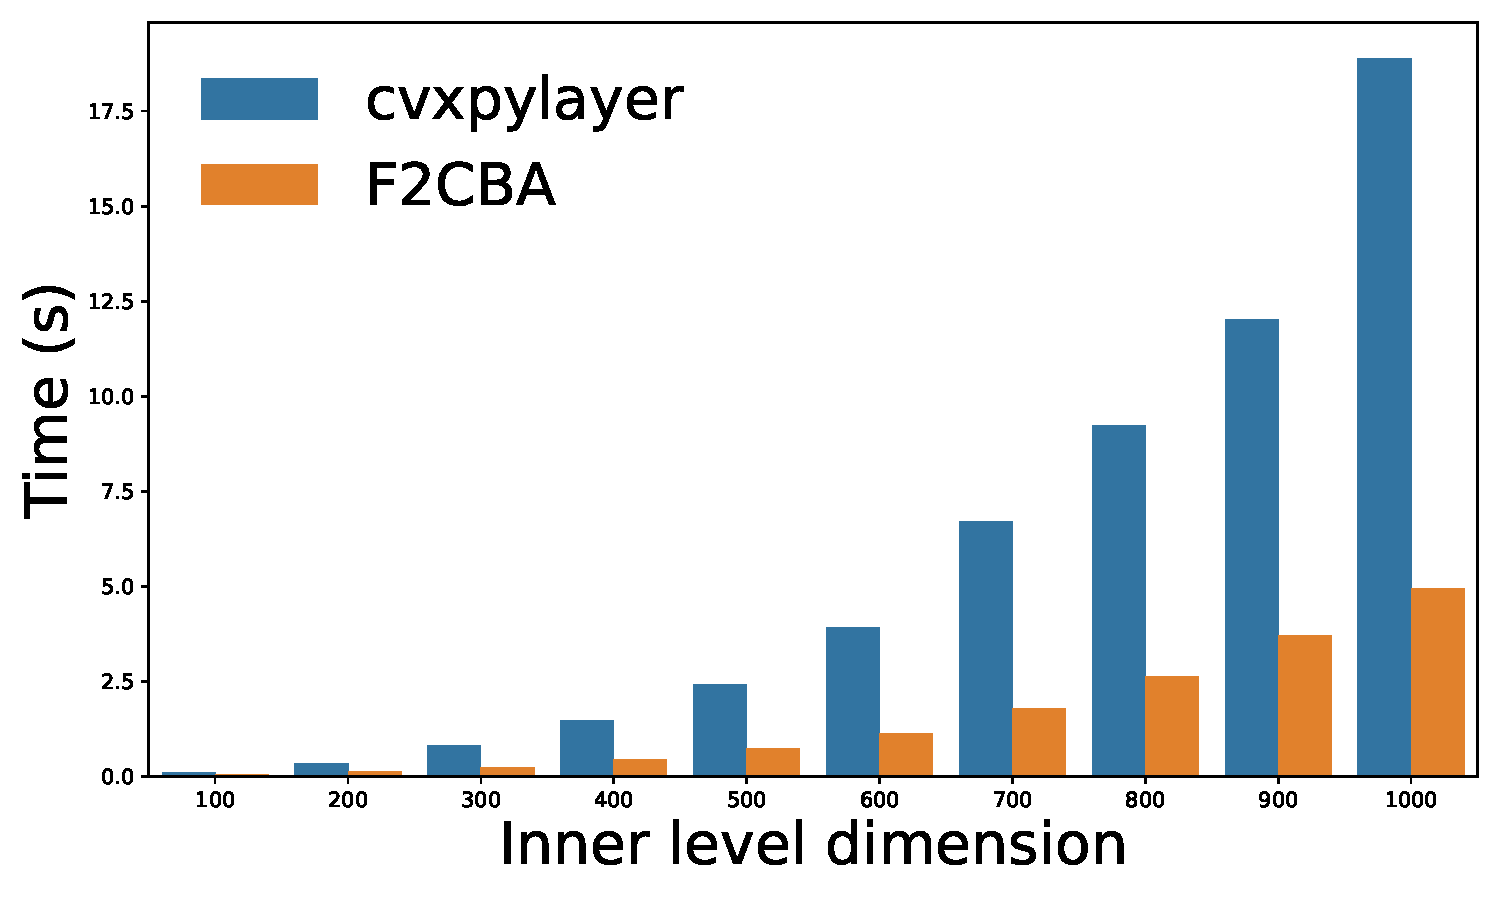
\includegraphics[width=\textwidth]{src/figures/time_results.pdf}
        \caption{Computation cost per gradient step of varying problem size $d_y$.}
        \label{fig:computation-comparison}
    \end{subfigure}
    \caption{We run \cref{alg: PIGD} using \cref{alg:inexact-gradient-oracle} on the bilevel optimization in the toy example in \cref{eqn:experiment-bilevel-optimization} with $d_x = 100$, $d_y = 200$, $n_{\text{const}} = d_y / 5$, and accuracy $\alpha = 1$. \cref{fig:convergence-comparison}, \cref{fig:convergence-comparison-2}, \cref{fig:computation-comparison} vary \# of iterations, gradient exactness $\alpha$, and $d_y$, respectively, to compare the performance under different settings.}
    % Figure~\ref{fig:convergence-comparison} shows that \cref{alg: PIGD} converges in the same rate as CvxpyLayer, while the gradient errors at each iteration are plotted in the colorful bars and are mostly below $\alpha = 0.1$ as guaranteed. Figure~\ref{fig:convergence-comparison-2} shows the convergence under different gradient inexactness $\alpha$. Figure~\ref{fig:computation-comparison} shows the computation cost of both methods under different lower level problem size $d_y$.}
    \label{fig:three graphs}
\end{figure}

We randomly generate the following constrained bilevel optimization problems. 
\begin{align*}\numberthis\label[prob]{eqn:experiment-bilevel-optimization}
     & \mbox{minimize}_{x} ~  c^\top y^* + 0.01 \norm{x}^2 + 0.01 \norm{y^*}^2 ~\text{ subject to } ~ y^* = \argmin_{y: h(x,y) \leq 0} \frac{1}{2} y^\top Q y + x^\top P y, 
\end{align*}
% \begin{align}\label{}
%     \min\nolimits_{x} \quad & \\
%     \text{s.t.} \quad & \nonumber
% \end{align}
where $h_i(x,y) = x^\top A_i y - x^\top b_i ~\forall i \in [K]$ are $K$ bilinear constraints. The PSD matrix $Q \in \reals^{d_y \times d_y}$, $c \in \reals^{d_y}$, $P \in \reals^{d_x \times d_y}$, and constraints $A_i \in \reals^{d_x \times d_y}$, $b_i \in \reals^{d_x}$ are randomly generated from normal distributions (cf. \cref{appendix:experiment-setup}).
We compare our \cref{alg: PIGD} with a non-fully first-order method implemented using \texttt{cvxpyLayer}~\cite{agrawal2019differentiable}. Both algorithms use Adam~\cite{kingma2014adam} to control the learning rate in gradient descent. All the experiments are averaged over ten random seeds.

% \paragraph{Convergence and computation comparisons:} 
\looseness=-1\cref{fig:convergence-comparison} shows that  
% compares the convergence of both methods. We can see that 
both the algorithms converge to the same optimal solution, while the fully first-order method is slightly more stable. Simultaneously, the colorful bars represent the gradient difference between two methods, showing the inexactness of gradient.
\cref{fig:convergence-comparison-2} additionally varies the inexactness to demonstrate its impact to convergence. One can find that too accurate gradient may also harm the convergence due to instability from poor condition numbers.
\cref{fig:computation-comparison} compares the computation cost of different lower level problem size $d_y$. Our fully first-order method significantly outperforms the differentiable optimization method in computation cost.


% \section{Applications} <- we'll get to these for the final manuscript



\bibliography{reference}
\bibliographystyle{icml2023}


%%%%%%%%%%%%%%%%%%%%%%%%%%%%%%%%%%%%%%%%%%%%%%%%%%%%%%%%%%%%%%%%%%%%%%%%%%%%%%%
%%%%%%%%%%%%%%%%%%%%%%%%%%%%%%%%%%%%%%%%%%%%%%%%%%%%%%%%%%%%%%%%%%%%%%%%%%%%%%%
% APPENDIX
%%%%%%%%%%%%%%%%%%%%%%%%%%%%%%%%%%%%%%%%%%%%%%%%%%%%%%%%%%%%%%%%%%%%%%%%%%%%%%%
%%%%%%%%%%%%%%%%%%%%%%%%%%%%%%%%%%%%%%%%%%%%%%%%%%%%%%%%%%%%%%%%%%%%%%%%%%%%%%%
\newpage
\appendix
\onecolumn
\section{Appendix}
\section{Random Ideas}
\subsection{Multi-objective Optimization Formulation}
The above bilevel optimization problem is equivalent to the following multi-objective optimization problem with an additional constraint.

\begin{align}
    \min_{\mechanism, \decision, \newdecision} & \quad \objective(\mechanism, \decision) ~ \text{and} ~ g(\mechanism, \newdecision) \\
    \text{s.t.} & \quad \decision = \newdecision \\ 
    & \quad \decision, \newdecision \in \Decision \\
    & \quad \mechanism \in \Mechanism
\end{align}


One of the most commonly used solutions to multi-objective optimization problem is to apply a weighted sum to multiple objectives to reduce to a single-objective optimization problem:

\begin{align}
    \min_{\mechanism, \decision, \newdecision} & \quad \objective(\mechanism, \decision) + w g(\mechanism, \newdecision) \\
    \text{s.t.} & \quad \decision = \newdecision \\
    & \quad \mechanism \in \Mechanism
\end{align}
where the weight $w$ is a hyper-parameter that can be tuned.
\textcolor{red}{Jimmy: I wonder if some strong regularity condition is required for existence of some $\omega$ to make it work. For the simple Bilevel optimization problem, a sufficiently large $\omega$ should be good.}


\subsection{Nonsmooth formulations}

Considering Eq.~\ref{eqn:two_constraints}, one can replace the two constraints $g(x,y)\leq g^*(x),~h(x,y)\leq0$ by the single constraint 
\[
c(x,y):=\max\{g(x,y)-g^*(x),h(x,y)\}\leq 0~.
\]
Note that whenever $g,h$ are $L$-Lipschitz and $\alpha$-strongly convex, then so is $c$, so good properties (other than smoothness) are preserved. This reduces the Lagrangian based analyses to a single multiplier, which seems good. Also note that we need to evaluate now the gradient of $c$, but this is possible whenever we have 0th+1st order access to $g,g^*,h$, since $\partial \max\{f_1,f_2\}=\mathrm{conv}\{\nabla f_i:f_i\mathrm{~attains~the~max}\}$.



Unrelated but also useful in this context, is that we can probably reduce the dimension dependence of \cite{chen2023bilevel} from $d^{3/2}$ to $d$. Their algorithm uses the gradient-free method of \cite{lin2022gradient} which suffers from a $d^{3/2}$ dependence, while they extend the analysis to hold for inexact zero-order oracles. Using instead the algorithm from \cite{kornowski2023algorithm} would reduce the dimension-dependence to $d$, if we show that this algorithm works with inexact oracles as well. The heart would be showing that \citep{cutkosky2023optimal} works under biased oracles. For a very concise analysis of that algorithm, I recommend the blog post: https://truenobility303.github.io/Optimal-NSNC/ (+ run through google translate if needed).

\subsection{Possibly using prior work via prox point method?}
The work of \cite{sabach2017first} provides an  algorithm for $\min_{x\in \arg\min f(x) + g(x)} \omega(x),$ where $f$ is smooth convex, $g$ is nonsmooth convex, and $\omega$ is smooth and convex. In particular, they prove convergence to an $\epsilon$-additive solution in both the outer and inner level problems at an iteration cost of $\epsilon^{-1}$, with a prox operation per iteration. Currently, it's not entirely clear to me if they allow any $g$ or only prox-friendly $g$. Can we use $g(x)= \delta_{h(x)\leq 0}$ (i.e., the indicator of the desired constraint set) and apply \cite{sabach2017first} directly? Their algorithm requires the use of the prox operator; specifically, to apply their algorithm as a blackbox, we need to understand to what accuracy they need to compute $\min_{x: h(x) \leq 0} \|u-x\|_2^2$ for some fixed $u$. Note that \cite{beck2014first} solves the constrained bilevel problem but seem to be limited to  the constraint set being ``prox-friendly''. Can we extend this to the general (strongly convex) $h$ case? Does \cite{sabach2017first} extend to $\omega$ not strongly convex; they seem to use properties of the resolvent of the gradient, which perhaps has extensions in the weakly convex settings. Also note that \cite{jiang2023conditional} improves upon \cite{sabach2017first}. 

%%%%%%%%%%%%%%%%%%%%%%%%%%%%%%%%%%%%%%%%%%%%%%%%%%%%%%%%%%%%%%%%%%%%%%%%%%%%%%%
%%%%%%%%%%%%%%%%%%%%%%%%%%%%%%%%%%%%%%%%%%%%%%%%%%%%%%%%%%%%%%%%%%%%%%%%%%%%%%%


\end{document}


% This document was modified from the file originally made available by
% Pat Langley and Andrea Danyluk for ICML-2K. This version was created
% by Iain Murray in 2018, and modified by Alexandre Bouchard in
% 2019 and 2021 and by Csaba Szepesvari, Gang Niu and Sivan Sabato in 2022.
% Modified again in 2023 by Sivan Sabato and Jonathan Scarlett.
% Previous contributors include Dan Roy, Lise Getoor and Tobias
% Scheffer, which was slightly modified from the 2010 version by
% Thorsten Joachims & Johannes Fuernkranz, slightly modified from the
% 2009 version by Kiri Wagstaff and Sam Roweis's 2008 version, which is
% slightly modified from Prasad Tadepalli's 2007 version which is a
% lightly changed version of the previous year's version by Andrew
% Moore, which was in turn edited from those of Kristian Kersting and
% Codrina Lauth. Alex Smola contributed to the algorithmic style files.
